\documentclass[xcolor=svgnames,ngerman]{beamer} %svgnames import a bunch of colors
%to make black and white paste ", blackandwhite" inside brackets above (for transparencies)
\usetheme{Stockton}

\usepackage[utf8]{inputenc}
\usepackage[ngerman]{babel}
\usepackage{csquotes}
% \usepackage{epsfig} %for figures
\usepackage{xcolor} %for color
\usepackage{amssymb}

\newcommand{\arr}[0]{$\rightsquigarrow${}{}}


\definecolor{hughesblue}{rgb}{.9,.9,1} %A blue I like to use for highlighting, matches Hughes Hallet's book


% \usepackage{minted} %Code highlighting

\usepackage{caption} %Mehrseitige Listings mit Caption

\usepackage{color}

\usepackage{gnuplottex}

% Minted shortcuts
% \newmintedfile{java}{linenos=true,tabsize=4,frame=single,baselinestretch=1,fontsize=\footnotesize}
% \newminted{java}{linenos=true,tabsize=4,frame=single,baselinestretch=1,fontsize=\footnotesize}


\definecolor{dkgreen}{rgb}{0,0.6,0}
\definecolor{gray}{rgb}{0.5,0.5,0.5}
\definecolor{mauve}{rgb}{0.58,0,0.82}
\setbeamercovered{transparent}
\logo{\includegraphics[height=1cm]{imgs/logo_uni.png}} % comment out this line if you do not have the pacific-seal file}

\title[Projektname: Subtitel \insertframenumber/
\inserttotalframenumber]{~ Projektname: Subtitel \\ sub sub titel} %the [whatever] appears in the footer on the right


\author{Max Mustermann} %the [whatever] appears in the footer on the left

\date{1. Januar 1970}
\newcommand\titlegraphicii[1]{\def\inserttitlegraphicii{#1}}
\titlegraphicii{}
\begin{document}

\begin{frame}
\vbox{}
   {\usebeamercolor[fg]{titlegraphic}\inserttitlegraphic\hfill\inserttitlegraphicii\par}
  \begin{centering}
    \begin{beamercolorbox}[sep=8pt,center]{institute}
      \usebeamerfont{institute}\insertinstitute
    \end{beamercolorbox}
    \begin{beamercolorbox}[sep=8pt,center]{title}
      \usebeamerfont{title}\inserttitle\par%
      \ifx\insertsubtitle\@empty%
      \else%
        \vskip0.25em%
        {\usebeamerfont{subtitle}\usebeamercolor[fg]{subtitle}\insertsubtitle\par}%
      \fi%     
    \end{beamercolorbox}%
    \vskip1em\par
    \begin{beamercolorbox}[sep=8pt,center]{date}
      \usebeamerfont{date}\insertdate
    \end{beamercolorbox}%\vskip0.5em
    \begin{beamercolorbox}[sep=8pt,center]{author}
      \usebeamerfont{author}\insertauthor
    \end{beamercolorbox}
  \end{centering}
\small
{Lehrstuhl f"ur Fachrichtung: Schwerpunkt tolle Sachen\par}
Pr"ufer: Prof. Dr. Max Mustermann\par\medskip
\end{frame}

% Was ist OSMAR
\section{Grundlagen}

\subsection{Projekttitel}

\begin{frame}[fragile]
\frametitle{Was ist Projekt?}
  \begin{itemize}
    \item Projekt = Arbeit + Thema
    \item Lorem
    \item +Ipsum: 
    \begin{itemize}
      \item Sub
      \item Sub
    \end{itemize}
  \end{itemize}
\end{frame}

{
\usebackgroundtemplate{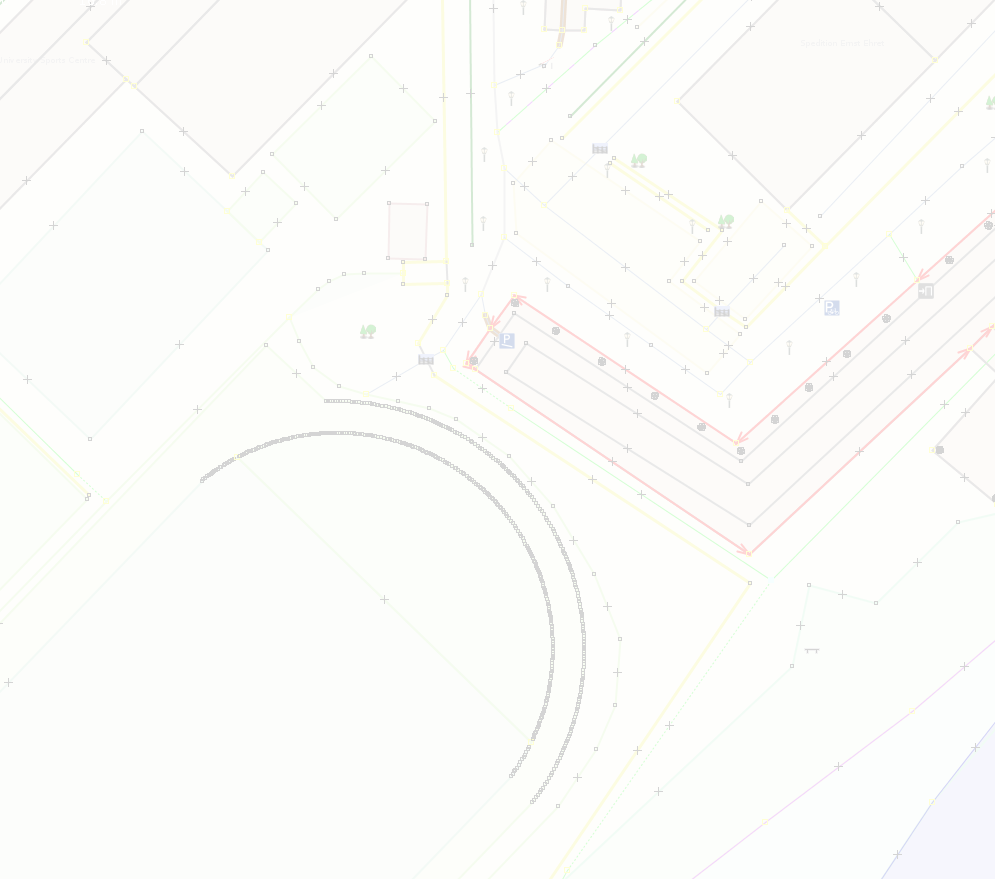
\includegraphics[width=\paperwidth]{imgs/pr_bg.png}}
\subsection{Lorem}
\begin{frame}[fragile]
\frametitle{Lorem?}
  \begin{itemize}
    \item Ipsum
  \end{itemize}
\end{frame}
}


\subsection{Demo}
\begin{frame}[fragile]
\frametitle{Projekt in Action}
\begin{center}
  \LARGE{Demo}
\end{center}
\end{frame}


\subsection{Sensoren}
\begin{frame}[fragile]
\frametitle{Tr"agheit}
\begin{figure} 
\begin{gnuplot}[terminal=pdf]
set terminal pdf size 4,2
set format y "%g°"
set format x "%g"
set title 'Trägheit'
set xlabel "Zeit in Millisekunden"
set ylabel "Delta Rotation"
set datafile sep ','
set decimalsign '.'

set yr [-0.15:+0.15]
xbase=0; ybase=0.7
set xr [0:100]
plot 'plots/plot.csv' u (x=$1-xbase):(y=($2-ybase)*-1) title "", 3 title "" lt rgb "blue", -3 title "3 Grad" lt rgb "blue"
\end{gnuplot}
\end{figure} 
\end{frame}


\section{Fazit}

\subsection{Fazit}
\begin{frame}[fragile]
\frametitle{}
  \begin{itemize}
    \item Voll toll
  \end{itemize}
\end{frame}

\begin{frame}[fragile]
\frametitle{}
  \begin{itemize}
    \item Hintergrund AR: CC BY-SA 3.0
    \item \arr URL
  \end{itemize}
\end{frame}

\frame {
  \frametitle{Fragen?}
  \LARGE{Herzlichen Dank f"ur Ihre Aufmerksamkeit}
  \LARGE{Fragen?}
}
\end{document}